\documentclass[conference]{IEEEtran}
\IEEEoverridecommandlockouts
% The preceding line is only needed to identify funding in the first footnote. If that is unneeded, please comment it out.
\usepackage{cite}
\usepackage{amsmath,amssymb,amsfonts}
\usepackage{algorithmic}
\usepackage{graphicx}
\usepackage{textcomp}
\usepackage{xcolor}
\def\BibTeX{{\rm B\kern-.05em{\sc i\kern-.025em b}\kern-.08em
    T\kern-.1667em\lower.7ex\hbox{E}\kern-.125emX}}
\begin{document}

\title{Identifying Giants and Dwarfs through Machine Learning\\
{\footnotesize \textsuperscript}
}
\author{\IEEEauthorblockN{José Moreira}
\IEEEauthorblockA{\textit{Dep. de Eletrónica, Telecomunicações e Informática}\\
\textit{Universidade de Aveiro)}\\
Aveiro, Portugal \\
jcristianosm@ua.pt}
\and
\IEEEauthorblockN{Bruno Aguiar}
\IEEEauthorblockA{\textit{Dep. de Eletrónica, Telecomunicações e Informática} \\
\textit{Universidade de Aveiro}\\
Aveiro, Portugal \\ 
brunoaguiar@ua.pt}
}

\maketitle

\begin{abstract}
Serves this document as a report on the first project of the class Machine Learning. The main objective is to perform a Stellar Classification (binary) by identifying Giants and Dwarfs using different classification methods such as Logistic Regression, Neural Networks and Support Vector Machines (SVM).
\end{abstract}

\vspace{5mm}

\begin{IEEEkeywords}
Machine Learning, Binary Classification, Logistic Regression, Neural Networks, Support Vector Machines
\end{IEEEkeywords}

\section{Introduction}
\par Stellar Classification is the classification of stars based on their spectral characteristics.  Electromagnetic radiation from the star is analyzed by splitting it with a prism or diffraction grating into a spectrum exhibiting the rainbow of colors interspersed with spectral lines. Each line indicates a particular chemical element or molecule, with the line strength indicating the abundance of that element. 

\par To distinguish if a star is a Giant or a Dwarf, we need to understand the classification mechanism that is currently used, which is the Morgan-Keenan (MK) System. MK System uses the letters O, B, A, F, G, K, M, with O being the hottest and M the coolest, and each letter has subclasses assigned to it, using the arabic numerals, 0-9, being 0 the hottest and 9 the coolest. Later on, the System was expanded to include classes for other stars, such as D for white dwarfs and S and C for carbon stars. A luminosity class was also added, using roman numerals and is based on the width of certain absorption lines in the star’s spectrum which vary with the density of the atmosphere and so distinguish giant stars from dwarfs. Luminosity class I is used for supergiants, class II for bright giants, class III for regular giants, class IV for sub-giants, class V for main-sequence stars, class VI for sub-dwarfs, and class VII for white dwarfs[1]. 
\par Other relevant features for the classification are the use of the Visual Apparent Magnitude of the Star, the Distance Between the Star and the Earth and the B-V color index. \par The Visual Apparent Magnitude of the Star is a measure of the brightness of a star observed from Earth. Star's apparent magnitude depends on its intrinsic luminosity, its distance from Earth, and any extinction of the object's light caused by interstellar dust along the line of sight to the observer. The B-V Color Index describes the color of the star and it ranges between zero or negative for an hot (blueish) star and 2.0 for a cold star. 
\par With these features we can create a fourth one, the Absolute Magnitude of the star, which is given by the equation \( M = m + 5(log_{10}^p+1) \), where \( M \) means the absolute magnitude,\( m \) means the visual apparent magnitude and \( p \) means the stellar parallax, also known as the distance from Earth, in a more simplified way.  


\section{Dataset}

To be able to execute this project, we used the 
\textbf{\textit{Star Dataset: Stellar Classification [Beginner]}}[2] that congregates six features of 3642 stars. Those features are Vmag - Visual Apparent Magnitude of the Star, Plx - Distance between the Star and the Earth, e\_Plx - Standard error of Plx, B-V - Color Index, SpType - Spectral Type and Amag - Absolute Magnitude of the Star. Besides those features, the dataset also contains the classification of all the 3642 stars. It is important to note that a full feature (\textit{SpType}) was removed from the project, as it was the classification mechanism to identify between a Giant and a Dwarf used to generate the \textit{TargetClass}. After said removal, it was analysed the presence of outliers, to understand if those values could affect the performance of any activity. It was found that they generally contribute to a good perform of the binary classification, except the ones in the e\_Plx column as they mean an error on the measures of the "Plx" column. Those outliers can be removed from the dataset as soon as they are greather than the standard deviation for that column. The following graph let us visualize such outliers: \\

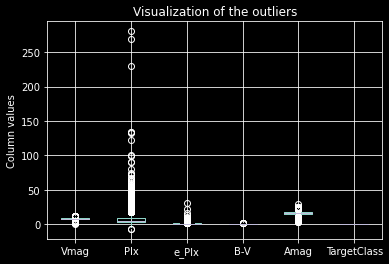
\includegraphics[scale=0.55]{outliears.png}
\caption{Figure 1 - Outliers}

\par


\section{Feature Normalization and Creation}
\subsection{Feature Clipping}
After some testing, it was decided there were some values that were way to low, or way to high that would stop any progress, and therefore, the first step that was made was to find those values and remove the entire correspondent row from the dataset, thus starting the data normalization by removing data that had too much error. We have a specific column that give us the standard error of the samples in the dataset, the e\_Plx column, so we have done this by automatically removing the rows that had a value 1.4 times higher than the standard deviation of that row, limiting the data to $N\sigma$ with $N = 1.4$. With this done, we were finally able to visualize pretty much all of the data in the dataset, however there were still some details missing, forcing a full data normalization. 
\par
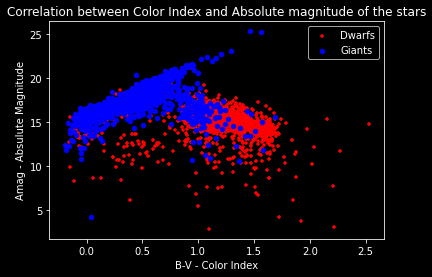
\includegraphics[scale=0.55]{vizdata.png} 
\caption{Figure 2 - Data Represented}
\par
\subsection{Feature Normalization}
The first approach, was to use the normalization Z Normalization (known also as Standardization, or Z-score) method, but that still resulted in some very high values that would incapacitate further algorithms. Finally, the used method was the Min-Max Normalization, also known as linear scaling, transforming all the values in the dataset in values between 0 and 1, given by the formula \( x = \frac{x - x_{min}}{x_{max} - x_{min}} \), allowing the ML algorithms to converge quickly without problems. It is also important to note that a full feature (\textit{SpType}) was removed from the project, as it was the classification mechanism to identify between a Giant and a Dwarf used to generate the \textit{TargetClass}.
\subsection{Feature Creation}
As stated before, the project has now five features to work with. However, creating features based on already existing ones will help increasing the accuracy on our algorithms classifications. Therefore, 72 features were created, each one based on 2 previous features, using a quadratic function that returned polynomial terms up to a given degree. Those features were than added to the dataset.



\section{Data Division}
One important aspect in machine learning is the bias-variance trade-off. A bias error is an error from a wrong assumption in the learning algorithm. A high bias can cause an algorithm to miss relevant relation between features, commonly called as underfitting. The variance is an error originated from small fluctuation in the training dataset, causing the algorithm to originate wrong outputs, commonly called as overfitting. To prevent this issues, and accomplish the best results, the data was divided in 3 new sets, a training set, used to train our models, a validation as it provides an unbiased evaluation of a model fit on the training dataset while tuning the model's hyperparameters and a testing set, the three used to compute and compare the model's accuracy and Score. 

\section{Logistic Regression}
Regarding classification methods, we started by using Logistic Regression. To be implemented, it required the use of Sigmoid  \( f(x) = \frac{1}{1+e^-x}\), a Cost Function and Gradient Descend with Ridge Regression (\(\frac{\lambda}{2m}\sum_{j=1}^{n}\theta^2_j\)) to provide regularization, in case it was needed. We opted to analyse the accuracy of the model with careful methodologies to diagnose the bias or the variance of the model, like Learning Curve and Validation Curve. The learning curve provide us the accuracy of the model over different batches of training samples, while the Validation Curve do the same, but over different hyper parameters values instead of different training sets. They are both helpful to assay the model is biased or not. They compute internally a confusion matrix to get the True Positives and Negatives, as well as False Positives and Negatives. With those values we compute the accuracy of the classification problem with the following formula \(Accuracy = \frac{TP+TN}{TP+TN+FP+FN}\). Starting with the Learning Curve, it provides us with the following graph:
\par
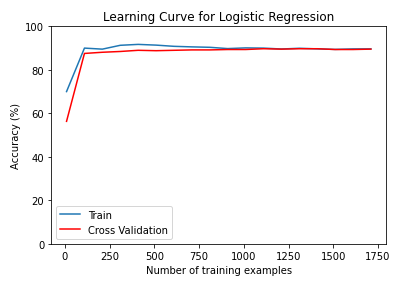
\includegraphics[scale=0.6]{LearningCurve.png}
\caption{Figure 3 - Learning Curve}
\par
This allows us to conclude that there is no overfitting or underfitting, since the accuracy goes up really quick, stabilizing at around 90\% and not dropping while the number of training examples adds up. 
\par
Concerning the Validation Curve, that plots the score over a varying hyper parameter, it will help us choose the best value for the regularization parameter \(lambda\) and helps confirming the results in the previous Curve, regarding the occurrence of bias and/or variance. Said curve is represented in the following graph:
\par
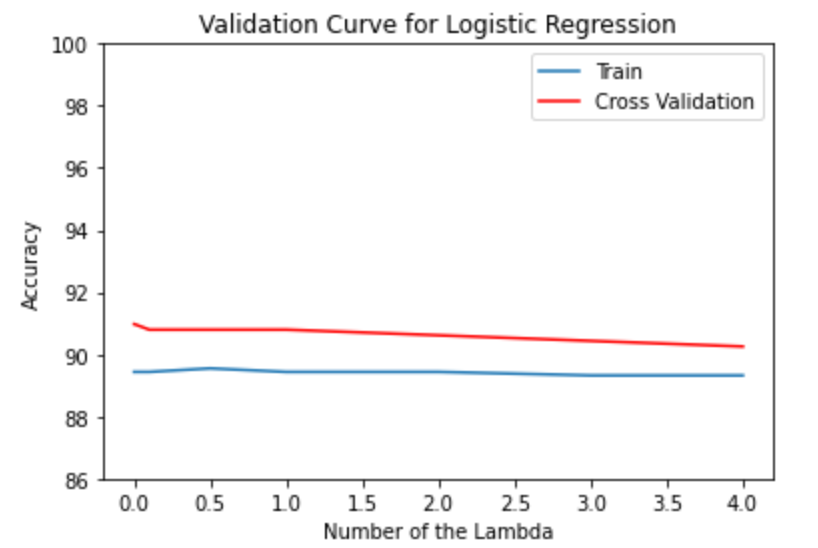
\includegraphics[scale=0.6]{Screenshot 2021-05-06 at 21.33.42.png}  
\caption{Figure 4 - Validation Curve}
\par
This allows us to conclude that the best \(lambda\) to use is, most of the times, 0, meaning that there is no need to do any regularizations, and some rare times some regularization is needed, due to the way the training sets and testins sets shuffle. This also confirms that there is no occurrence of underfitting or overfitting.
It is also important to report that these methods achieve an accuracy of about 89-92\%, floating in between as the 3-Way-Split method shuffle the data within, in each execution. We also performed a F1-Score to see how much penalty the model received from its output extremes. The penalty was around 2\% of less real accuracy.  

\section{Neural Networks}
The second method used was Neural Networks. It is known that Logistic Regression it not very efficient for complex non linear models, and despite it being good enough for this problem, since it has a close to 90\% accuracy, we would like to know how much of and upgrade the Neural Networks would provide. For starters, we used the Neural Network Cost Function with Backpropagation provided in class, with a Sigmoid Gradient obtained with \(g'(z) = \frac{d}{dz}g(z) = g(z)(1-g(z))\). To randomly initialize weights, we also used the method provided in class, that is \(\epsilon_{init} = \frac{\sqrt{6}}{\sqrt{L_{in} + L_{out}}}\) where \(L_{in}\) is the length of the input layer and \(L_{out}\) is the length of the output layer of the network. To calculate the Gradient Descent, we made some adaptions on what was provided in class, in order to add Adaptive Learning Rate, with the goal of minimizing the objective function of a network, and Momentum, that accumulates the gradient of the previous steps to determine the next one. Because of time constraints, we did not perform a more rigorous test for the model (like F1-Score or the K-Fold) rather than comparing both train and test sets. With the testing done, it is possible to confirm that better results were in fact obtained, since it gained an improvement of around 1-\% over the Logistic Regression model. Although we had some improvement over the Logistic Regression, we have concluded that, because of the overhead and time that the Neural Network consumes, it's very likely that it's not worth it to choose it over the Logistic Regression, for such problem. It was also possible to conclude that the Cost Function using Gradient Descent declines as the number of Iterations rises, until it stabilizes at around 0.3, as shown in the following graph: 
\par
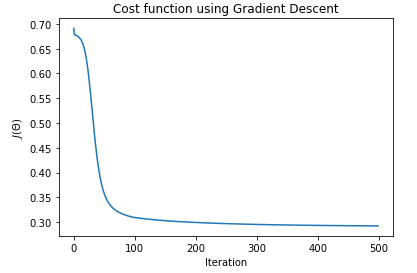
\includegraphics[scale=0.6]{CostFunctionNN.png}
\caption{Figure 5 - Cost Function}
\par

\section{SVM}
The last method used to classify the type of stars was the SVM, or Support-Vector Machines. SVMs work by training examples to points in space, dividing the space in two areas, meaning when something is to be classified, the place where the representation point appears corresponds to the category the method assumes it belongs. The method used was based in what we learnt in class, with some adaptations to turn it in to something easier to re-use[3]. To configure our classifier, many kernels were testes, and "poly" was the one that provided better results, therefore it is the only used from now on. Since we were only able to train with two features, we designed two graphs, one with the features we has most success with, and one with other features to compare the difference in the Score of both. In the first example, we had the following graph:
\par
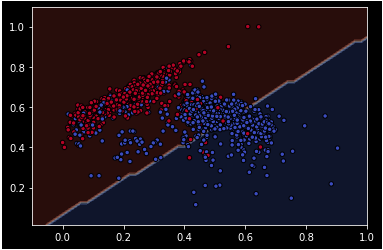
\includegraphics[scale=0.6]{SVM1.png}
\caption{Figure 6 - SVM Best Graph}
\par
In this example, a score of 87.288\% was achieved. In the second example, with regular features, we obtained the following graph:
\par
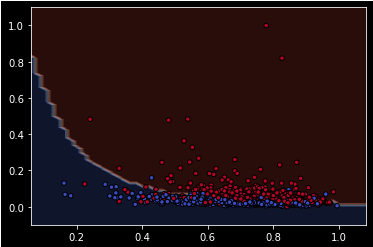
\includegraphics[scale=0.6]{SVM2.png}
\caption{Figure 7 - SVM Graph}
\par
In this example, an 81.695\% was achieved, confirming our expectations regarding the importance of the features. 

\section{KFold}
To cross validate our testing, we implemented KFold, to divided the data in training sets and testing sets. We used 5 splits in the data, meaning we calculated the Balanced Accuracy and the F1 Score of 5 different sets, followed by calculating the average of those values. On average, our SVM classification method achieved 89.888\% and 89.89\% in Balanced Accuracy in Train set and Test set respectively, and 88.409\% and 88.367\% in F1 Score, also Train set and Test set respectively. Since it is required False Positives, False Negatives, True Positives and True Negatives to calculate these values, we also got the confusion matrix's for both sets. \\
\par 
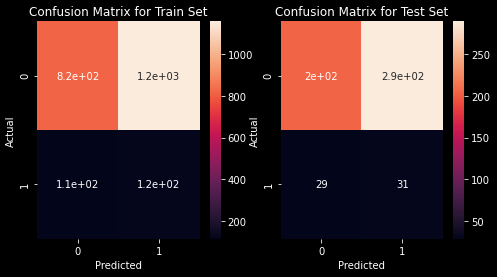
\includegraphics[scale=0.5]{CMatrixSVM.png}
\caption{Figure 8 - SVM Confusion Matrix}
\par

\section{Conclusion}
Regarding work distribution, Bruno Aguiar has done Neural Networks, the F1-Score and Matrix Confusion of Logistic Regression, José Moreira has done SVM, and everything else was done by both students simultaneously. Concerning the results obtained, they were fairly expected. All three methods constantly hit close to 90\% accuracy, with the Logistic Regression one excelling at 92\% at times. With that said, and considering the resources consumed to implement all methods, it is safe to assume that the Logistic Regression one is the most adequate to deal with this problem.
It is also important to state that the dataset is randomly divided in training set and testing set, therefore, the results presented in this report may not be exacly the ones the presented in the Jupyter Notebook file. 
\begin{thebibliography}{00}
\bibitem[1]{b1} 
"Stellar classification" (April 2021). Wikipedia 
\bibitem[2]{b2} https://www.kaggle.com/vinesmsuic/star-categorization-giants-and-dwarfs/code
\bibitem[3]{b3}
https://stackoverflow.com/questions/51297423/plot-scikit-learn-sklearn-svm-decision-boundary-surface
\end{thebibliography}

	

\end{document}
